This section provides an overview of \mfix's Discrete Element Modelling (DEM)
abilities. \mfix's DEM simulations retain all the functionality of MFIX-DEM.
\mfix\ can be run in both a pure granular (particles only) mode
as well as a particle fluid-coupling mode. In the latter case, \mfix\ models
the fluid phase as a continuum and models the
particles of the solid phase individually. This approach supports a wide range
of customization for particle dynamics, including multiple particle collision
forces. For more information on the DEM capabilities of \mfix\
see \demdoc\ on the MFIX Documentation webpage at
{\url{https://mfix.netl.doe.gov/download/mfix/mfix_current_documentation/dem_doc_2012-1.pdf/}}.

\section{Overview}

\begin{figure}
    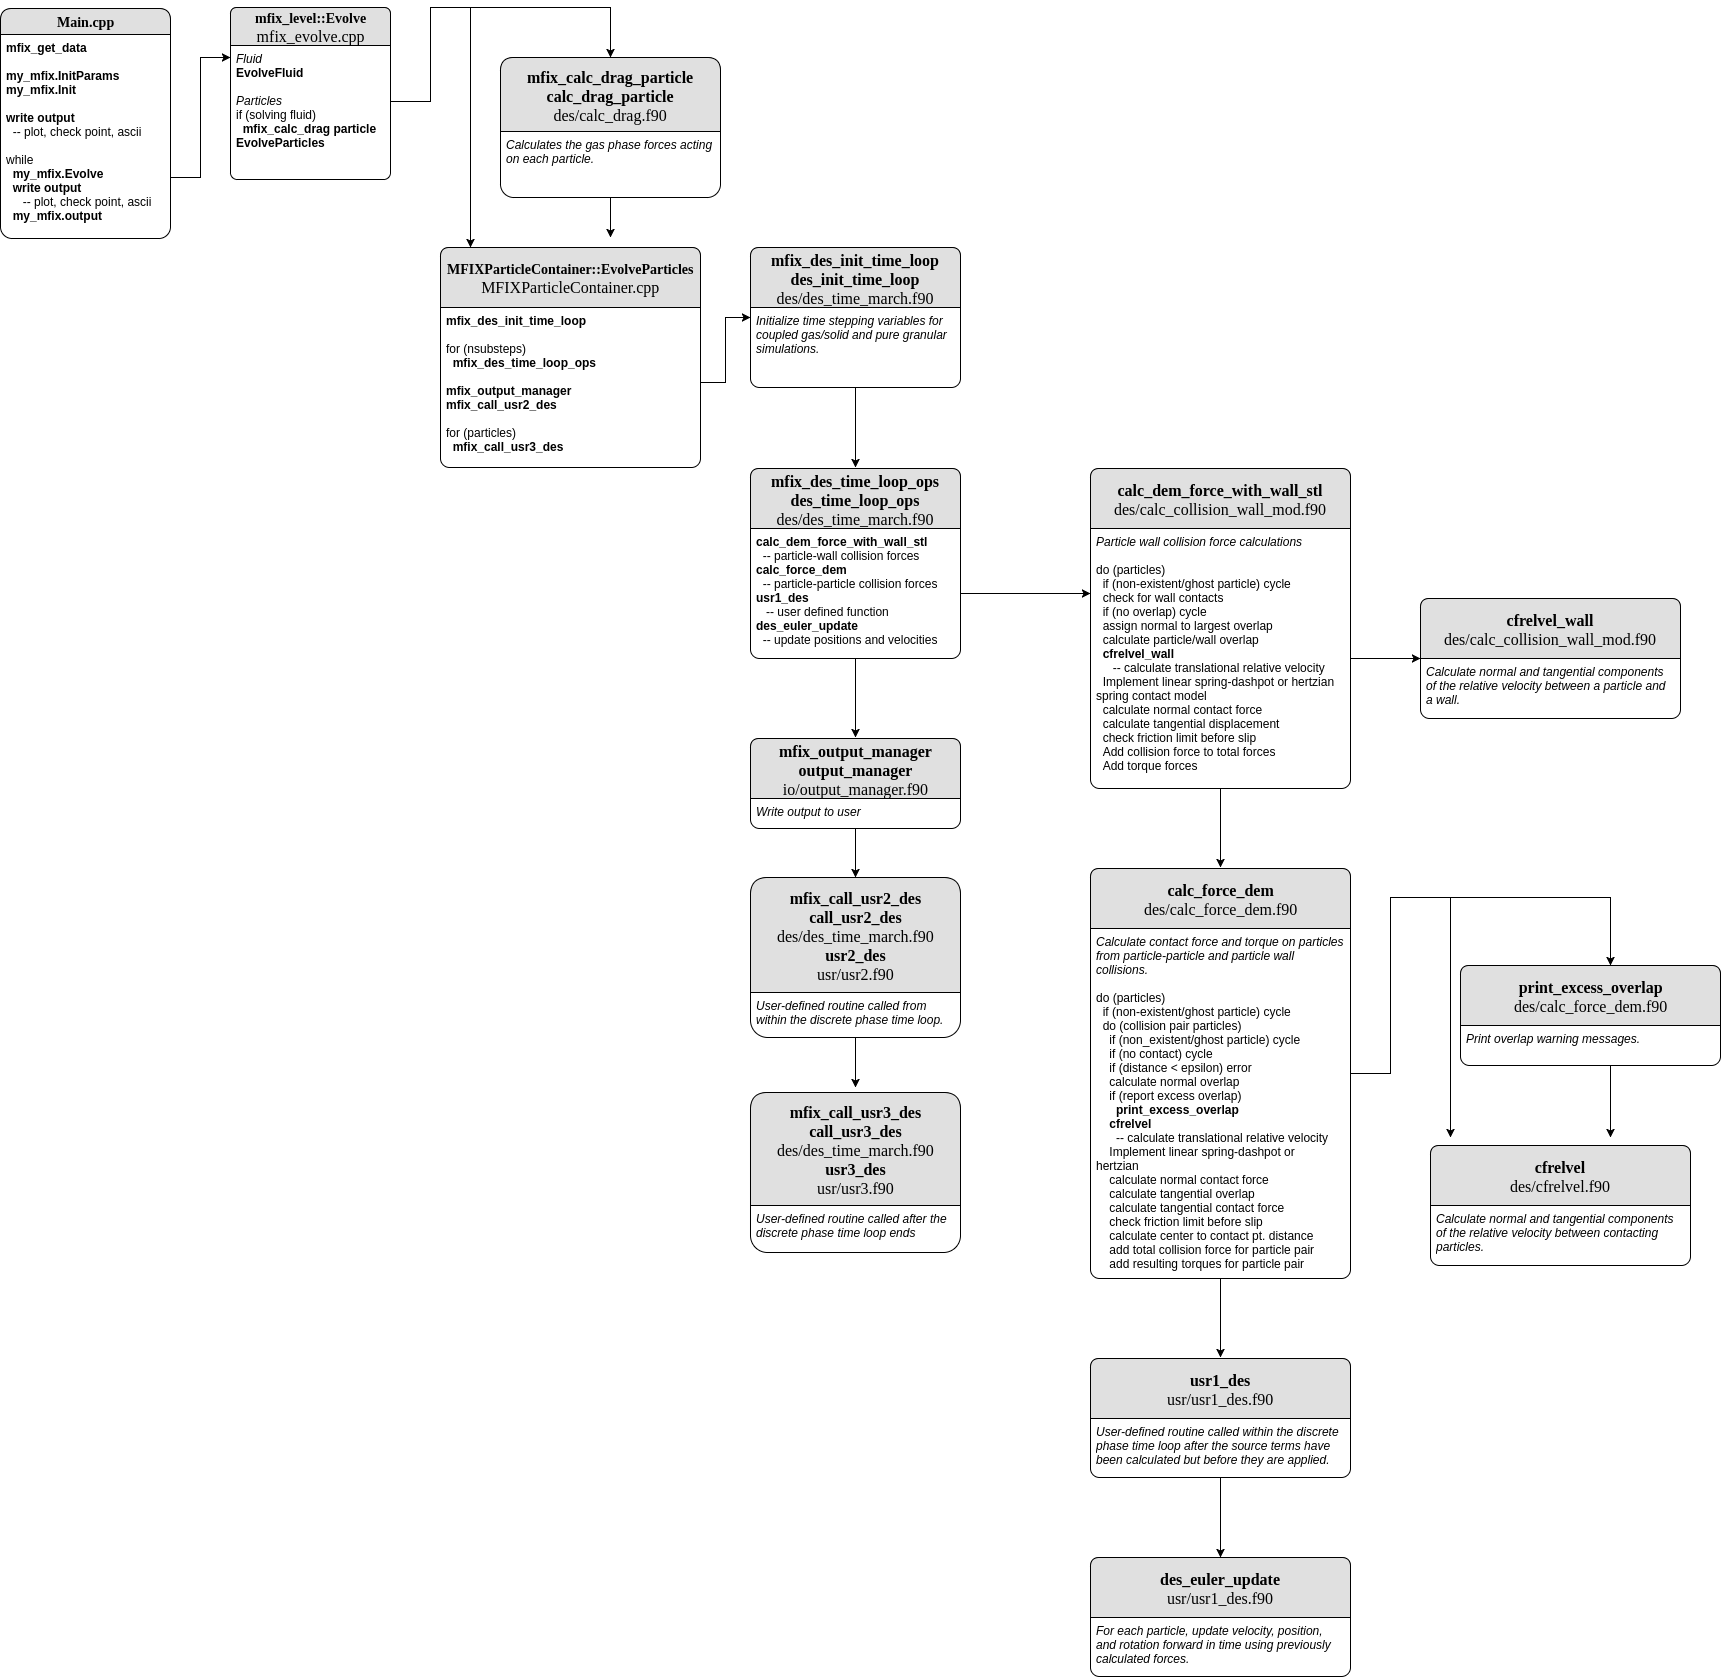
\includegraphics[width=\linewidth,natwidth=800, natheight=600]{./Particles/MFIX-Particle-Diagram.png}
    \caption{Particle Routines Flowchart}
    \label{fig:pflowchart}
\end{figure}

\mfix\ retains all the functionality of MFIX-DEM. A detailed discription of the
particles dynamics can thus be found in \demdoc.
In addition, figure \ref{fig:pflowchart} provides a visual representation
of the particle routines in \mfix.

\section{Equations}

\mfix\ natively supports one soft-sphere contact force model, the linear
spring-dashpot model. The linear spring-dashpot model is discussed in
section {\bf 2.2.1: Contact Forces} of \demdoc.


\section{Initializing the Particles}

Particles are initialized via the ASCII file {\sf particle\_input.dat}. The
first line of the file states the number of particles. The following lines
contain the details of each particle in the format: \\

{\sf phase x y z radius density $\omega_x$ $\omega_y$ $\omega_z$}  \\

\noindent
where {\sf $\omega_x$, $\omega_y$, $\omega_z$} refer to the angular velocities
 of the particle. All quantities are entered as real numbers separated by a
single space except {\sf phase} which takes an integer value.


%\subsection{Random placement}
%
%The option to initialize particle with random placement will be enabled in
%the future.



\section{Time Stepping}

\mfix\ currently uses a first-order forward in-time Euler method to advance
the particles. A discussion of the advantages, limitations and details of this
aproach is available in section {\bf 3.1: Time Integration} of \demdoc.

\section{Output Format}

Simulation output parameters are set in the inputs file that is passed to mfix
as the first argument when the program in called. This section will refer
to this file as {\sf inputs}. Output options that can be set in this file are
shown in table \ref{table:amropts}.

\begin{table}
\begin{center}
  \begin{tabular}{||c| l||}
    \hline
    Command & Function \\ [0.5ex]
    \hline\hline
    {\sf amr.plot\_int} & Sets the plot frequency in terms of fluid simulation\\
                        & time steps, i.e. {\sf amr.plot\_int=2} will output a
                          plot file \\
                        & every two time steps. \\
     \hline
    {\sf amr.plot\_file} & Sets the plot filename prefix. \\
     \hline
  \end{tabular}
\end{center}
\caption{\amrex\ Output Options}
\label{table:amropts}
\end{table}

\subsection{Checkpoint Files}

All particle information is stored in a binary file within each checkpoint
directory. This format is designed for being read by the code at restart rather
than for diagnostics. Full details on checkpoints files are available in the
\amrex\ User's Guide under section {\bf 4.17.2: Checkpoint File}.


\subsection{Plot Files}

\mfix\ uses \amrex's framework for plot files. Visualization of particles is
most readily achieved with the ParaView software. See \amrex User's Guide section
{\bf 9.3: ParaView} for instructions on how to generate particle plot files.


\subsection{ASCII Particle Files}
Writing ASCII particle files is explained in \hyperref[sec:AsciiFiles]{Writing ASCII
Particle Files}.

%\subsection{Run-time Data Logs}


%\noindent {\bf amr.data\_log = }{\em log\_file}  \\



%\subsection{Run-time Screen Output}
